% Stanford University PhD thesis style -- modifications to the report style
% This is unofficial so you should always double check against the
% Registrar's office rules
% See http://library.stanford.edu/research/bibliography-management/latex-and-bibtex
% 
% Example of use below
% See the suthesis-2e.sty file for documentation
%
\documentclass{report}
\usepackage{suthesis-2e}
\usepackage{graphicx}
\usepackage{verbatim} % for block comment
\usepackage{color}   % May be necessary if you want to color links
\usepackage{hyperref}
\usepackage{textcomp}
\usepackage[backend=bibtex,style=ieee,natbib=true]{biblatex} % Use the bibtex backend with the authoryear citation style (which resembles APA)
\addbibresource{../src/mybib.bib} % The filename of the bibliography
\hypersetup{
colorlinks=true, %set true if you want colored links
linktoc=all,     %set to all if you want both sections and subsections linked
linkcolor=black,  %choose some color if you want links to stand out
}
\dept{Electronic and Information Engineering}

\begin{document}
    \title{Fast Depth Coding in 3D-HEVC\\
    Using Deep Learning}
    \author{Zhen-xiang WANG}
    \principaladviser{Yui-Lam Chan}
    \beforepreface
    \prefacesection{Abstract}
    With the rising popularity of the high definition videos, the new standard
    termed High Efficiency Video Coding (HEVC) for compressing videos in a more
    efficient way comparing with previous standards, such as H.264/AVC, has
    emerged under the efforts from the Joint Collaborative Team on Video
    Coding (JCT-VC).
    In the meanwhile, five extensions of the HEVC standard, comprising
    Format Range Extension (RExt), Scalability Extension (SHVC),
    Multi-view Extension (MV-HEVC), 3D Extension (3D-HEVC),
    Screen Content Coding Extension (SCC),  have been finalized
    from 2014 to 2016 to support fulfill extra requirements in various
    scenarios.
    3D Video applications are attracting more interests
    \prefacesection{Acknowledgments}
    I would like to thank...
    \afterpreface

    \chapter{Introduction}\label{ch:chapter1} % For referencing the chapter elsewhere, use \ref{Chapter1}

%----------------------------------------------------------------------------------------
Video is the medium to record, copy, playback, broadcast
and display the motion images in an electronic style~\parencite{RN190}.
Watching videos is becoming an important way for our entertainment as well
as education.
The high definition (HD) and ultra high definition (UHD) video
are increasingly demanding nowadays.
People prefer videos with higher definitions than those with lower
resolutions because the former one provides much better viewing experience.
However, challenges emerged for delivering videos with high definition.
HD videos typically contain much more information in every picture frame than the
standard definition videos.
More data needs to be squeezed into the same capacity for transmission.
For example, the uncompressed video with the dimension 720 x 480 at 30 frames
per second requires 0.03 gigabytes per second, while the uncompressed video with
the dimension 2880 x 2048 at 120 frames per second requires 2.12 gigabytes per
second.
Since bit rate is proportional to system bandwidth for
transmission~\parencite{RN191}, and expanding the bandwidth in a large scale is
too expensive, the significantly increased bit rate
for transmitting the video data is becoming one of the
major obstacles for HD video services.\\
\newline
To cope with the growing need for higher compression of moving
pictures~\parencite{RN193}, Joint Collaborative Team on Video
Coding (JCT-VC)~\parencite{RN192} has developed the High Efficiency Video
Coding standard which is the newest international video coding standard for
substantially ameliorate the compression performance against the previous
standards.
Comparing with the H.264 Advanced Video Compression Standard~\parencite{RN194},
the H.265 High Efficiency Video Coding Standard provides fifty percent bit rate
reduction while maintaining the objective video quality at the same level.\\
\newline
While Two-dimensional video is the most common video type,
Three-dimensional (3D) video has been brought to market via lots of ways,
including Blu-Ray disc, cable and satellite transmission, terrestrial
broadcast, and streaming or downloading from the Internet~\parencite{RN118}.
3D video provides the perception of depth information which augments
the vividness of the video contents.
Currently most 3D videos in the market are using stereo display technology.
Two similar views, one for left eye, the other for right eye, are presented
at the same time with the multiplexing techniques enabling the
adjustments of video geometry information~\parencite{RN196} to provide
the 3D effect.
Figure~\ref{fig:stereo-display} illustrates the typical system structure for
transmitting videos targeting stereo display.
It can be observed that there exists a displacement between the
two views.
The green vertical left margins of the red rectangles in the two views
at encoder side are different.
Such a displacement is the visual disparity for 3D perception.
Stereoscopic videos~\parencite{RN153} have
achieved great profitability for movie theatres in recent years.
For example, IMAX 3D has became the most popular one that offering
the immersing multimedia experiences around the world.
Special 3D glasses are needed for watching the IMAX 3D movies.
The current 3D film industry is very successful in terms of attracting
customers, however, it is not the end of the story.
Myopic people do not like to wear one more pair of glasses when
watching 3D movies.
Some people will experience discomfort after wearing the 3D glasses for a
period of two hours.
Autostereoscopic multi-view technology~\parencite{RN153} is coming to our rescue.
No glasses are needed if Autostereoscopic videos can
substitute the Stereoscopic videos.
The Autostereoscopic multi-view display demands more than two
views for audience to view the 3D contents
without extra eye glasses.
The visual quality of
the Autostereoscopic display is highly correlated to the number of views
that can be provided in the receiver side.
Due to limited available bandwidth, transmitting arbitrary number of views
is not practical.
Researchers have proposed a new format which is making use of limited number
of view and their associated depth maps~\parencite{RN44}.
The typical system structure for using this new format to compress and supply 3D video
resources is shown in figure~\ref{fig:SS-MVD}.
\begin{figure}
    \centering
    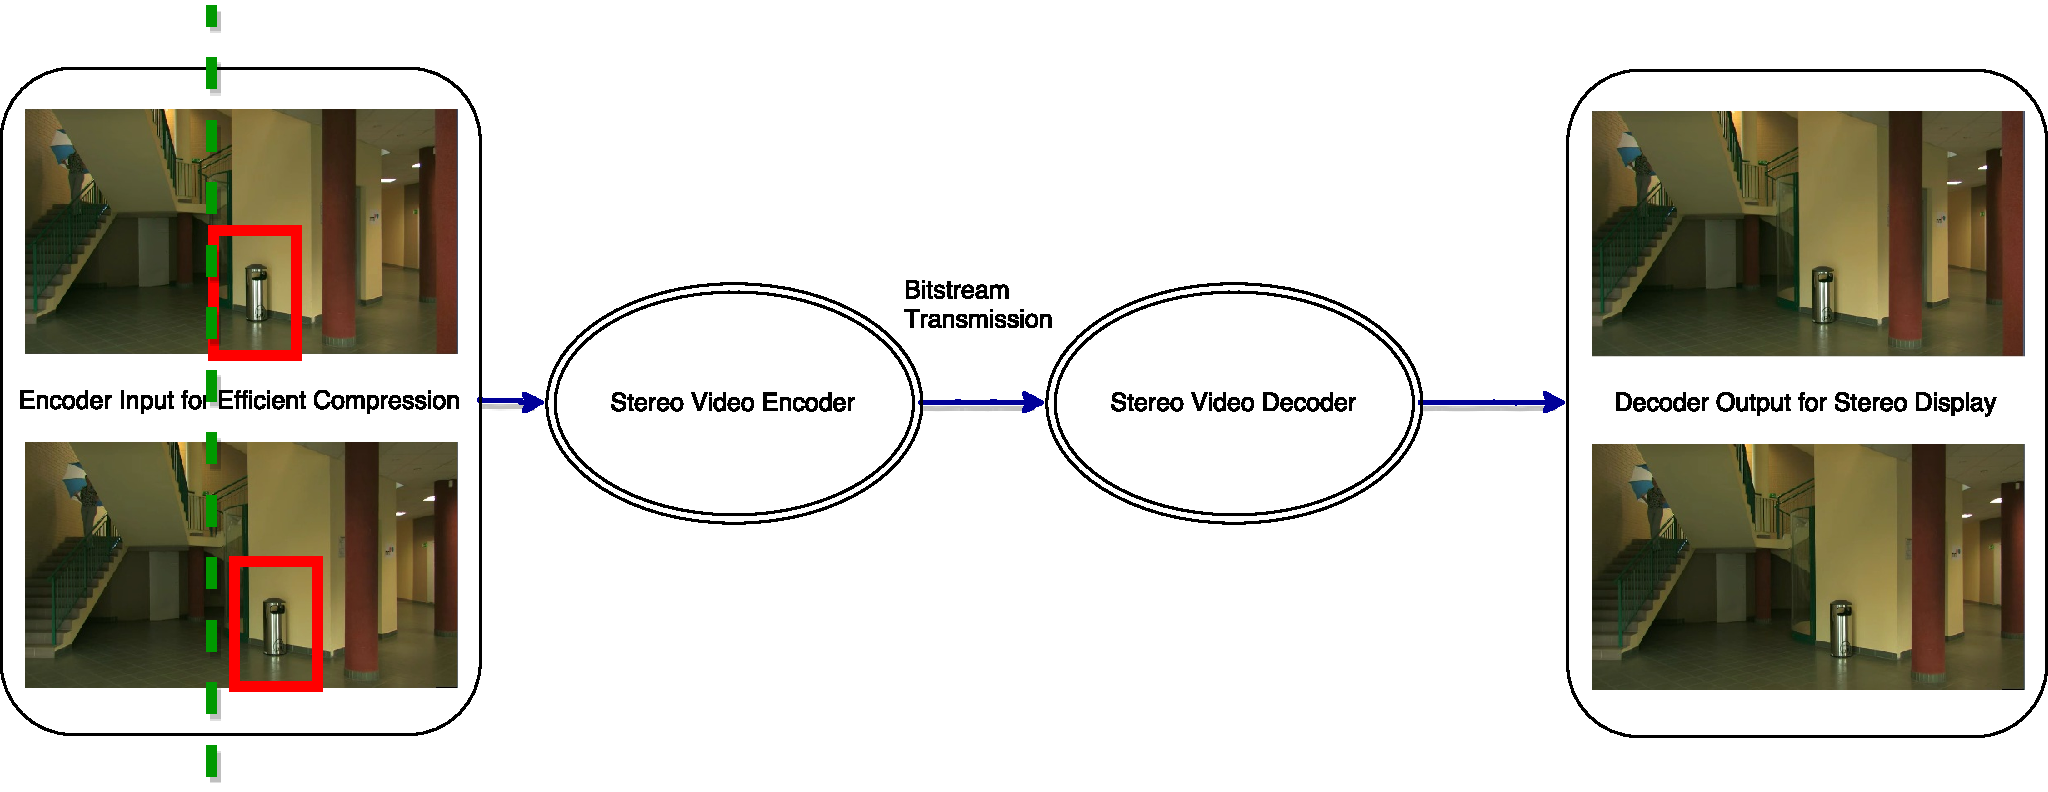
\includegraphics[width=\textwidth,height=\textheight,keepaspectratio]{Figures/StereoDisplay}
%        \decoRule
    \caption[System Structure for transmitting videos targeting stereo display]{System Structure for transmitting videos targeting stereo display.}
    \label{fig:stereo-display}
\end{figure}
An enormous amount of views in the medium positions which are able to
guarantee the high quality of the 3D video can be synthesized from
\begin{figure}
    \centering
    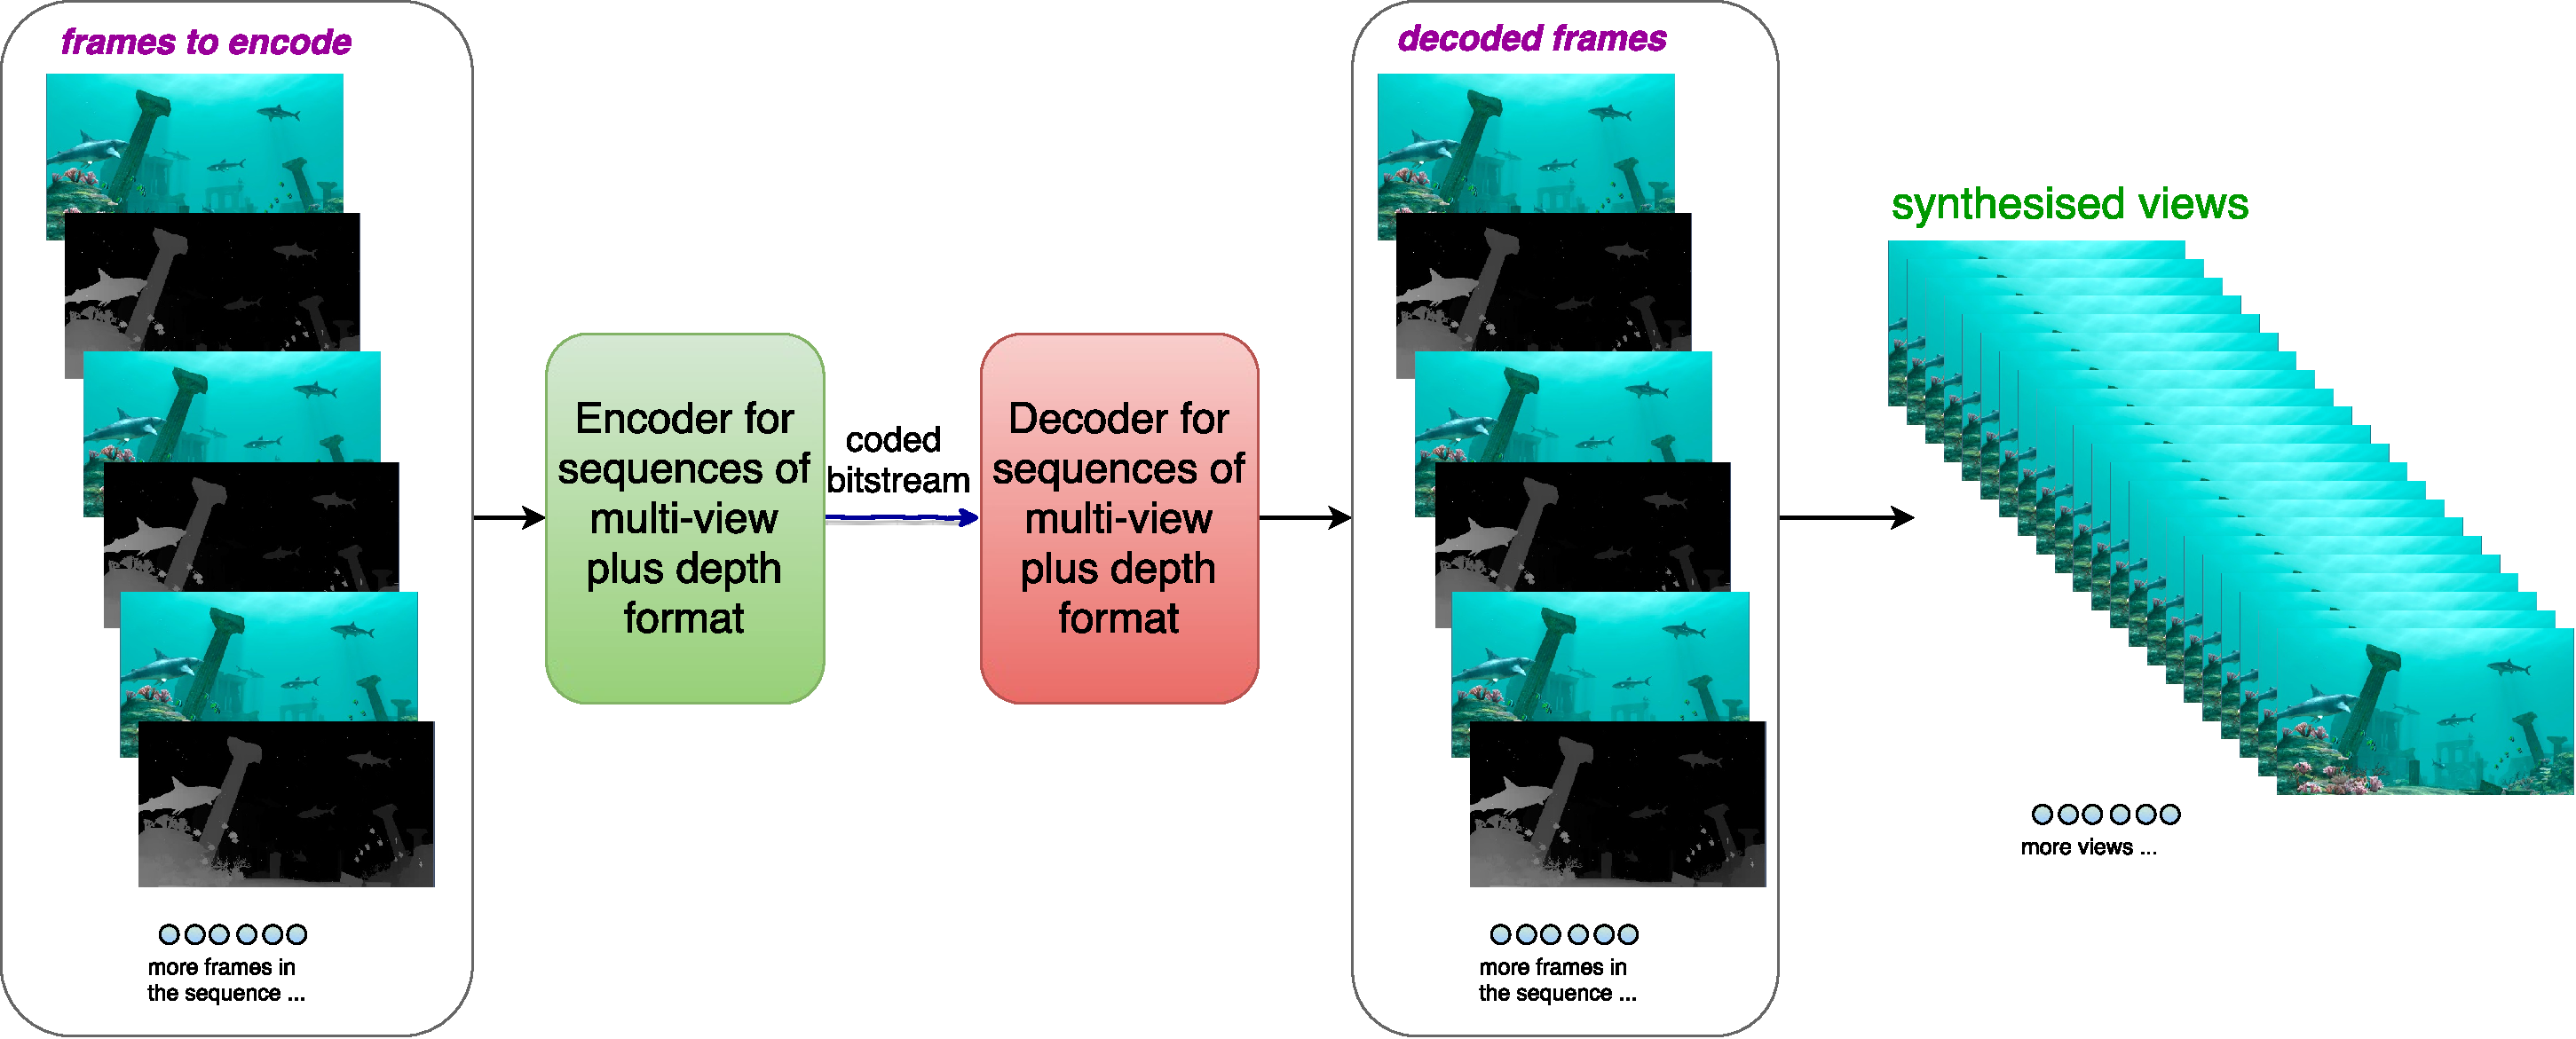
\includegraphics[width=\textwidth,height=\textheight,keepaspectratio]{Figures/SystemStructureOf3DEncoder}
%        \decoRule
    \caption[System Structure for transmitting videos of Multi-view Plus Depth format]{System Structure for transmitting videos of Multi-view Plus Depth format.}
    \label{fig:SS-MVD}
\end{figure}
the decoded texture frames in combination with decoded depth maps.\\
%The multi-view plus depth format provides the functionality of synthesizing
%required number of views from texture views and associated depth maps.\\
\newline
To employ multi-view plus depth format for 3D video, efficient compressing
methods are desired, which has led to the 3D Video Coding Extension of the
High Efficiency Video Coding Standard (3D-HEVC) by the Joint Collaborative Team
on 3D Video Coding Extension Development (JCT-3V)~\parencite{RN195}.
The 3D Extension of the HEVC standard gives extra coding efficiency
for encoding a few texture views along with the corresponding depth maps by
using new tools which exploit the redundancies amongst
texture and depth views, and pay attention to the unique characteristics of
the depth maps, such as large homogeneous
regions separated by sharp boundaries~\parencite{RN47}.\\
\newline
Depth information measures of the distance between the object in the far position
and the object in the near position from a static viewpoint,
which is expressed in the format of depth map.
Instead of presenting depth maps directly to the viewer, views in the medium
positions are generated by Depth-Image-Based Rendering (DIBR) technique.
The qualities of the depth maps are vital to the DIBR process.
Corona artifacts (a.k.a. ringing artifacts) can be discovered in synthesized
views if the edge sharpness in depth maps can not be well
preserved.
Therefore, retaining the edge sharpness in depth map is the key to avoid the
artifacts in the synthesized views.
In 3D-HEVC, new intra-picture prediction and residual coding methods
have been applied to preserve the special properties of depth
map.
Depth Modelling Mode (DMM), which is one of the new intra-picture
prediction tools, is designed to provide much more granularity for
encoding the depth maps.
Wedgelet partition and contour partition for depth maps
are enabled by DMM1 and DMM4 separately.
%~\parencite{RN197}.

%introduce a little about depth map and their usage.
%mentioning iphonex true depth camera.
%draw the picture

%----------------------------------------------------------------------------------------

\section{Motivation and Contribution}\label{sec:motivation_and_contribution}
%fasdfasdfasdfasdfasdfasdf figure~\ref{fig:SS-MVD}
If you are
\begin{table}
    \label{tab:treatments}
    \centering
    \begin{tabular}{c r @{.} l}
        Pi expression       &
        \multicolumn{2}{c}{Value} \\
        \hline
        $\pi$               & 3&1416  \\
        $\pi^{\pi}$         & 36&46   \\
        $(\pi^{\pi})^{\pi}$ & 80662&7 \\
    \end{tabular}
    \caption{The effects of treatments X and Y on the four groups studied.}
\end{table}

\begin{table}
    \label{tab:tabular_example1}
    \centering
    \begin{tabular}[t]{|r|l|}
        \hline
        7C0 & hexadecimal \\
        3700 & octal \\
        \cline{2-2} 11111000000 & binary \\
        \hline
        \hline
        1984 & decimal \\
        \hline
    \end{tabular}
\caption{Just an example}
\end{table}

\begin{table}
    \label{tab:tabular_example2}
    \centering
    \begin{tabular}{|r|l|}
        \hline
        7C0 & hexadecimal \\
        3700 & octal \\
%        \cline{2-2}
%        11111000000 & binary \\
%        \hline
%        \hline
%        1984 & decimal \\
        \hline
    \end{tabular}
\caption{Basic Usage}
\end{table}

\begin{table}
    \label{tab:tabular_example3}
    \centering
    \begin{tabular}{|r|l|}
        \hline
        7C0 & hexadecimal \\
        \cline{1-2}
        3700 & octal \\
        \cline{2-2}
        11111000000 & binary \\
        \cline{1-2}
        11111000 & binary \\
%        \hline
%        \hline
%        1984 & decimal \\
        \hline
    \end{tabular}
\caption{horizontal lines extend over multiple columns}
\end{table}

\begin{table}
    \label{tab:tabular_example4}
    \centering
    \begin{tabular}{|p{4.7cm}|}
        \hline Welcome to Boxy's paragraph. We sincerely hope you'll all enjoy the show.\\
        \hline
    \end{tabular}
    \caption{define a special type of column which will wrap-around the text as in a normal paragraph}
\end{table}

\begin{table}
    \label{tab:tabular_example8}
    \centering
    \begin{tabular}{p{4.7cm}}
        \hline
        Welcome to Boxy's paragraph.
        We sincerely hope you'll all enjoy the show.\\
        \hline
    \end{tabular}
    \caption{define a special type of column which will wrap-around the text as in a normal paragraph}
\end{table}

\begin{table}
    \label{tab:tabular_example5}
    \centering
    \begin{tabular}{@{} l @{}}
        \hline Welcome to Boxy's paragraph. We sincerely hope you'll all enjoy the show.\\
        \hline
    \end{tabular}
    \caption{define a special type of column which will wrap-around the text as in a normal paragraph}
\end{table}

\begin{table}
    \label{tab:tabular_example6}
    \centering
    \begin{tabular}{l}
        \hline Welcome to Boxy's paragraph. We sincerely hope you'll all enjoy the show.\\
        \hline
    \end{tabular}
    \caption{define a special type of column which will wrap-around the text as in a normal paragraph}
\end{table}

\begin{table}
    \label{tab:tabular_example9}
    \centering
    \begin{tabular}{c c} \hline \multicolumn{2}{c}{Ene} \\ \hline Mene & Muh! \\ \hline \end{tabular}
    \caption{multicolumn command}
\end{table}

\begin{table}
    \label{tab:tabular_example10}
    \centering
    \begin{tabular}{c c c c c c}
        \hline
        sequence name &
        BD-BR &
        \multicolumn{4}{c}{Ene} \\
        \cline{3-6}
        {} & {} & Me & Muh & Me & Mu\\
        \hline
        Newspaper & 0.98\% & 22 & 33 & 44 & 66\\
    \end{tabular}
    \caption{multicolumn command}
\end{table}




%\begin{table}
%    \label{tab:treatments}
%    \centering
%    \begin{tabular}{c r @{.} l}
%        Pi expression       &
%        \multicolumn{2}{c}{Value} \\
%        \hline
%        $\pi$               & 3&1416  \\
%        $\pi^{\pi}$         & 36&46   \\
%        $(\pi^{\pi})^{\pi}$ & 80662&7 \\
%    \end{tabular}
%    \caption{The effects of treatments X and Y on the four groups studied.}
%\end{table}
%----------------------------------------------------------------------------------------

\section{Dissertation Outline}\label{sec:outline}




%\chapter{Introduction}\label{ch:chapter1} % For referencing the chapter elsewhere, use \ref{Chapter1}
%
%%----------------------------------------------------------------------------------------
%
%%----------------------------------------------------------------------------------------
%
%\section{Welcome and Thank You}\label{sec:welcome}
%Welcome to this \LaTeX{} Thesis Template, a beautiful and easy to use template for writing a thesis using the \LaTeX{} typesetting system.
%
%If you are writing a thesis (or will be in the future) and its subject is technical or mathematical (though it doesn't have to be), then creating it in \LaTeX{} is highly recommended as a way to make sure you can just get down to the essential writing without having to worry over formatting or wasting time arguing with your word processor.
%
%\LaTeX{} is easily able to~\parencite{RN93} professionally typeset documents that run to hundreds or thousands of pages long. With simple mark-up commands, it automatically sets out the table of contents, margins, page headers and footers and keeps the formatting consistent and beautiful. One of its main strengths is the way it can easily typeset mathematics, even \emph{heavy} mathematics. Even if those equations are the most horribly twisted and most difficult mathematical problems that can only be solved on a super-computer, you can at least count on \LaTeX{} to make them look stunning.
%
%%----------------------------------------------------------------------------------------
%
%\section{Welcome and Thanku}\label{sec:welome}
%Welcome to this \LaTeX{} Thesis Template, a beautiful and easy to use template for writing a thesis using the \LaTeX{} typesetting system.
%
%If you are writing a thesis (or will be in the future) and its subject is technical or mathematical (though it doesn't have to be), then creating it in \LaTeX{} is highly recommended as a way to make sure you can just get down to the essential writing without having to worry over formatting or wasting time arguing with your word processor.
%
%\LaTeX{} is easily able to professionally typeset documents that run to hundreds or thousands of pages long. With simple mark-up commands, it automatically sets out the table of contents, margins, page headers and footers and keeps the formatting consistent and beautiful. One of its main strengths is the way it can easily typeset mathematics, even \emph{heavy} mathematics. Even if those equations are the most horribly twisted and most difficult mathematical problems that can only be solved on a super-computer, you can at least count on \LaTeX{} to make them look stunning.
%
%%----------------------------------------------------------------------------------------
%
%\section{Welcome and ThYou}\label{sec:weome}
%Welcome to this \LaTeX{} Thesis Template~\parencite{Reference1}, a beautiful and easy to use template for writing a thesis using the \LaTeX{} typesetting system.
%
%If you are writing a thesis (or will be in the future) and its subject is technical or mathematical (though it doesn't have to be), then creating it in \LaTeX{} is highly recommended as a way to make sure you can just get down to the essential writing without having to worry over formatting or wasting time arguing with your word processor.
%
%\LaTeX{} is easily able to professionally typeset documents that run to hundreds or thousands of pages long. With simple mark-up commands, it automatically sets out the table of contents, margins, page headers and footers and keeps the formatting consistent and beautiful. One of its main strengths is the way it can easily typeset mathematics, even \emph{heavy} mathematics. Even if those equations are the most horribly twisted and most difficult mathematical problems that can only be solved on a super-computer, you can at least count on \LaTeX{} to make them look stunning.
%
%%----------------------------------------------------------------------------------------
%
%\section{Welcome and Thau}\label{sec:welcoe}
%Welcome to this \LaTeX{} Thesis Template, a beautiful and easy to use template for writing a thesis using the \LaTeX{} typesetting system.
%
%If you are
%\begin{table}
%
%    \label{tab:treatments}
%    \centering
%%    \begin{tabular}{l l l}
%%        \toprule
%%        \tabhead{Groups} & \tabhead{Treatment X} & \tabhead{Treatment Y} \\
%%        \midrule
%%        1 & 0.2 & 0.8\\
%%        2 & 0.17 & 0.7\\
%%        3 & 0.24 & 0.75\\
%%        4 & 0.68 & 0.3\\
%%        \bottomrule\\
%%    \end{tabular}
%    \begin{tabular}{c r @{.} l}
%        Pi expression       &
%        \multicolumn{2}{c}{Value} \\
%        \hline
%        $\pi$               & 3&1416  \\
%        $\pi^{\pi}$         & 36&46   \\
%        $(\pi^{\pi})^{\pi}$ & 80662&7 \\
%    \end{tabular}
%    \caption{The effects of treatments X and Y on the four groups studied.}
%\end{table}
%writing a thesis (or will be in the future) and its subject is technical or mathematical (though it doesn't have to be), then creating it in \LaTeX{} is highly recommended as a way to make sure you can just get down to the essential writing without having to worry over formatting or wasting time arguing with your word processor.
%
%\LaTeX{} is easily able to professionally typeset documents that run to hundreds or thousands of pages long. With simple mark-up commands, it automatically sets out the table of contents, margins, page headers and footers and keeps the formatting consistent and beautiful. One of its main strengths is the way it can easily typeset mathematics, even \emph{heavy} mathematics. Even if those equations are the most horribly twisted and most difficult mathematical problems that can only be solved on a super-computer, you can at least count on \LaTeX{} to make them look stunning.
%
%%----------------------------------------------------------------------------------------
%
%\section{Welcome and Tnk You}\label{sec:wlcome}
%Welcome to this \LaTeX{} Thesis Template, a beautiful and easy to use template for writing a thesis using the \LaTeX{} typesetting system.
%
%If you are writing a thesis.
%
%%\begin{verbatim}
%\begin{figure}
%    \centering
%    
\includegraphics{Figures/Electron}
%    %    \decoRule
%    \caption[An Electron]{An electron (artist's impression).}
%    \label{fig:Electron}
%\end{figure}
%%\end{verbatim}
%(or will be in the future) and its subject is technical or mathematical (though it doesn't have to be), then creating it in \LaTeX{} is highly recommended as a way to make sure you can just get down to the essential writing without having to worry over formatting or wasting time arguing with your word processor.
%
%\LaTeX{} is easily able to professionally typeset documents that run to hundreds or thousands of pages long. With simple mark-up commands, it automatically sets out the table of contents, margins, page headers and footers and keeps the formatting consistent and beautiful. One of its main strengths is the way it can easily typeset mathematics, even \emph{heavy} mathematics. Even if those equations are the most horribly twisted and most difficult mathematical problems that can only be solved on a super-computer, you can at least count on \LaTeX{} to make them look stunning.
%
%%----------------------------------------------------------------------------------------

%    \chapter{Conclusions}
    ...
%    \appendix
%    \chapter{A Long Proof}
    ...
    \printbibliography[heading=bibintoc]
\end{document}